\chapter{Celdifferentiatie: de skeletspiercel}\label{ch:b2:cell-differentiation}

Een vezel van je dijspier is één enkele cel van dertig centimeter lang,
met honderden kernen, van begin tot eind volgepakt met samentrekbare
staafjes die zo regelmatig liggen dat ze er onder de microscoop gestreept
uitziet. Ze begon als een groepje gewoon ogende cellen die uit een somiet
kropen, zich vermenigvuldigden, ophielden met delen, zich op een rij
zetten, versmolten, en enkele honderden genen aanschakelden die ze nooit
eerder hadden gebruikt. Elke cel van het lichaam heeft hetzelfde genoom;
een \omterm{def:b2:cell-differentiation:myogenesis}{spiervezel} is wat dat genoom doet wanneer één bepaalde
\omterm{prop:b2:cell-differentiation:transcriptional}{transcriptiefactor} wordt aangeschakeld. Dit hoofdstuk neemt de
skeletspiercel als uitgewerkt voorbeeld van \emph{\omterm{def:b2:cell-differentiation:differentiation}{differentiatie}} --- hoe
een cel een gespecialiseerde identiteit verwerft en behoudt --- en de
spiercel is daarvoor een goed voorbeeld, omdat de hoofdschakelaar bekend is,
de stappen in een schaaltje te volgen zijn, en de voltooide cel een
machine is waarvan de onderdelen zichtbaar zijn.

\section{Wat differentiatie is}

\begin{definition}[Differentiatie, determinatie, potentie]\label{def:b2:cell-differentiation:differentiation}
\index{differentiatie}\index{determinatie}\index{stamcel}\index{potentie}
Een cel is \emph{gedifferentieerd} wanneer ze het stabiele genpatroon ---
en dus de eiwitten, de vorm en de functie --- van één celtype tot expressie
brengt. Ze is \emph{gedetermineerd} (of vastgelegd) wanneer haar lot
vastligt hoewel haar differentiatie nog niet is begonnen: een \omterm{def:b2:cell-differentiation:myogenesis}{myoblast} ziet
eruit als een fibroblast, maar zal alleen spier maken. \emph{Potentie} is
het bereik aan typen dat een cel nog kan voortbrengen: \emph{totipotent}
(de zygote en de eerste blastomeren, die alles maken, de \omterm{def:b2:mammal-reproduction:placenta}{placenta}
inbegrepen), \emph{pluripotent} (de \omterm{def:b2:mammal-reproduction:implantation}{binnenste celmassa}, die elk weefsel van
het lichaam maakt), \emph{multipotent} (een stamcel van het bloed of van
spier, die de typen van één weefsel maakt), \emph{unipotent}. Een
\emph{stamcel} is een cel die zich deelt in een dochtercel die aan haarzelf
gelijk is en een die verder differentieert, wat de voorraad in stand houdt
en tegelijk het weefsel bevoorraadt. Differentiatie is in de meeste gevallen
geen verlies van genen maar een keuze tussen genen: het genoom van een
spierkern is volledig.
\end{definition}
\begin{proof}[Bewijsmateriaal]
Gurdon (1962) bracht de kern van een gedifferentieerde darmcel van een
kikkervisje over in een kikkerei waarvan de eigen kern was vernietigd; een
deel van de eieren ontwikkelde zich tot normale, vruchtbare kikkers. De
gedifferentieerde kern had geen van de genen verloren die nodig zijn om een
heel dier te maken; het cytoplasma van het ei had hem teruggezet. Dezelfde
ingreep met de kern van een melkkliercel in een schapenei leverde Dolly op
(1996), en het herprogrammeren van een huidfibroblast tot een pluripotente
\omterm{def:b2:cell-differentiation:differentiation}{stamcel} met vier \omterm{prop:b2:cell-differentiation:transcriptional}{transcriptiefactoren} (Yamanaka, 2006) toonde aan dat het
terugzetten met een handvol eiwitten kan.
\end{proof}

\begin{proposition}[Differentiatie is een kwestie van transcriptie]\label{prop:b2:cell-differentiation:transcriptional}
\index{transcriptiefactor}\index{hoofdregulator}
Het verschil tussen twee celtypen ligt in welke genen worden
overgeschreven. Een paar \emph{\omterm{prop:b2:cell-differentiation:transcriptional}{transcriptiefactoren}}, tot expressie gebracht
als antwoord op de inductieve signalen van
\cref{ch:b2:vertebrate-development}, binden aan de regelgebieden van
honderden doelgenen en schakelen die aan, terwijl de genen van andere
lotbestemmingen worden uitgeschakeld; en omdat zo'n factor gewoonlijk zijn
eigen gen activeert, houdt de toestand zichzelf in stand zodra hij is
bereikt. Voor sommige weefsels is één enkele factor een \emph{\omterm{prop:b2:cell-differentiation:transcriptional}{hoofdregulator}}
die volstaat om het lot op te leggen aan een cel van een ander type: \omterm{def:b2:cell-differentiation:myogenesis}{MyoD}
voor skeletspier, Pax6 voor het oog, Sox9 voor kraakbeen. De toestand wordt
verder gestabiliseerd door veranderingen in het chromatine --- methylering
van DNA, modificatie van histonen --- die de uitgeschakelde genen over de
delingen heen stil houden (de \emph{epigenetica} van het deel van jaar 3).
Een gedifferentieerde cel onthoudt dus wat ze is zonder enige verandering
in haar DNA-sequentie, en het geheugen is geschreven in het patroon van
factoren en chromatine, niet in de genen.
\end{proposition}

\section{De vorming van een spiervezel}

\begin{definition}[Myogenese]\label{def:b2:cell-differentiation:myogenesis}
\index{myoblast}\index{myotube}\index{spiervezel}\index{MyoD}
In het embryo worden cellen van het dermomyotoom van de somiet door
signalen uit de \omterm{prop:b2:vertebrate-development:neurulation}{neurale buis}, de chorda en het oppervlakte-ectoderm ertoe
aangezet de myogene factoren \emph{MyoD} en \emph{Myf5} tot expressie te
brengen: het zijn nu \emph{myoblasten}, gedetermineerd maar nog delend en
onopvallend van uiterlijk. Myoblasten migreren --- bijvoorbeeld de
ledemaatknoppen in --- en vermenigvuldigen zich zolang er groeifactoren
(FGF) aanwezig zijn. Wanneer die op raken, treden ze uit de celcyclus,
brengen ze een tweede factor, \emph{myogenine}, tot expressie, stellen ze
zich kop aan staart op en \emph{versmelten} ze: hun membranen vloeien samen
tot één lange \emph{myotube} met vele kernen op een rij. De myotube
schakelt de spiergenen aan --- actine, myosine, troponine, tropomyosine,
creatinekinase, de acetylcholinereceptor ---, bouwt het contractiele
apparaat en rijpt tot een \emph{spiervezel} waarvan de kernen aan de
rand liggen. Een vezel deelt zich nooit meer; een paar myoblasten blijven
er in rust naast liggen als \emph{satellietcellen}, de stamcellen die de
spier levenslang herstellen en laten groeien.
\end{definition}

\begin{omfigure}
\begin{tikzpicture}[every node/.style={font=\scriptsize}, >=stealth]
  % somite
  \draw[thick, fill=omProp!25] (0,0) ellipse (0.6 and 0.5); \node[below, align=center] at (0,-0.6) {somiet\\(dermomyotoom)};
  \draw[->, thick] (0.7,0) -- (1.6,0) node[midway, above=0.35cm, align=center] {inductie\\Wnt, Shh};
  % myoblasts dividing
  \foreach \p in {(2.2,0.3),(2.7,-0.3),(3.2,0.3),(3.7,-0.3)} \draw[thick, fill=omDef!25] \p ellipse (0.28 and 0.18);
  \node[below, align=center] at (3.0,-0.6) {myoblasten: MyoD, Myf5\\delen zolang er FGF is};
  \draw[->, thick] (4.1,0) -- (5.0,0) node[midway, above=0.45cm, align=center] {FGF weggenomen:\\myogenine,\\uit de cyclus};
  % aligned, fusing
  \foreach \x in {5.35,5.95,6.55,7.15} \draw[thick, fill=omDef!25] (\x,0) ellipse (0.3 and 0.16);
  \node[below, align=center] at (6.25,-0.6) {op een rij en versmelten};
  \draw[->, thick] (7.6,0) -- (8.5,0);
  % myotube
  \draw[thick, fill=omDef!15, rounded corners=6pt] (8.7,-0.3) rectangle (12.6,0.3);
  \foreach \x in {9.2,10.0,10.8,11.6,12.3} \fill[omDef!80!black] (\x,0) ellipse (0.13 and 0.08);
  \node[below, align=center] at (10.65,-0.6) {myotube: vele kernen,\\spiergenen aan, myofibrillen gebouwd};
\end{tikzpicture}

{\small Myogenese: geïnduceerde cellen van de somiet worden delende
\omterm{def:b2:cell-differentiation:myogenesis}{myoblasten}; wanneer de groeifactoren wegvallen, houden ze op met delen,
stellen ze zich op een rij en versmelten ze tot een meerkernige \omterm{def:b2:cell-differentiation:myogenesis}{myotube}
die de spiergenen aanschakelt.}
\end{omfigure}

\begin{omfigure}
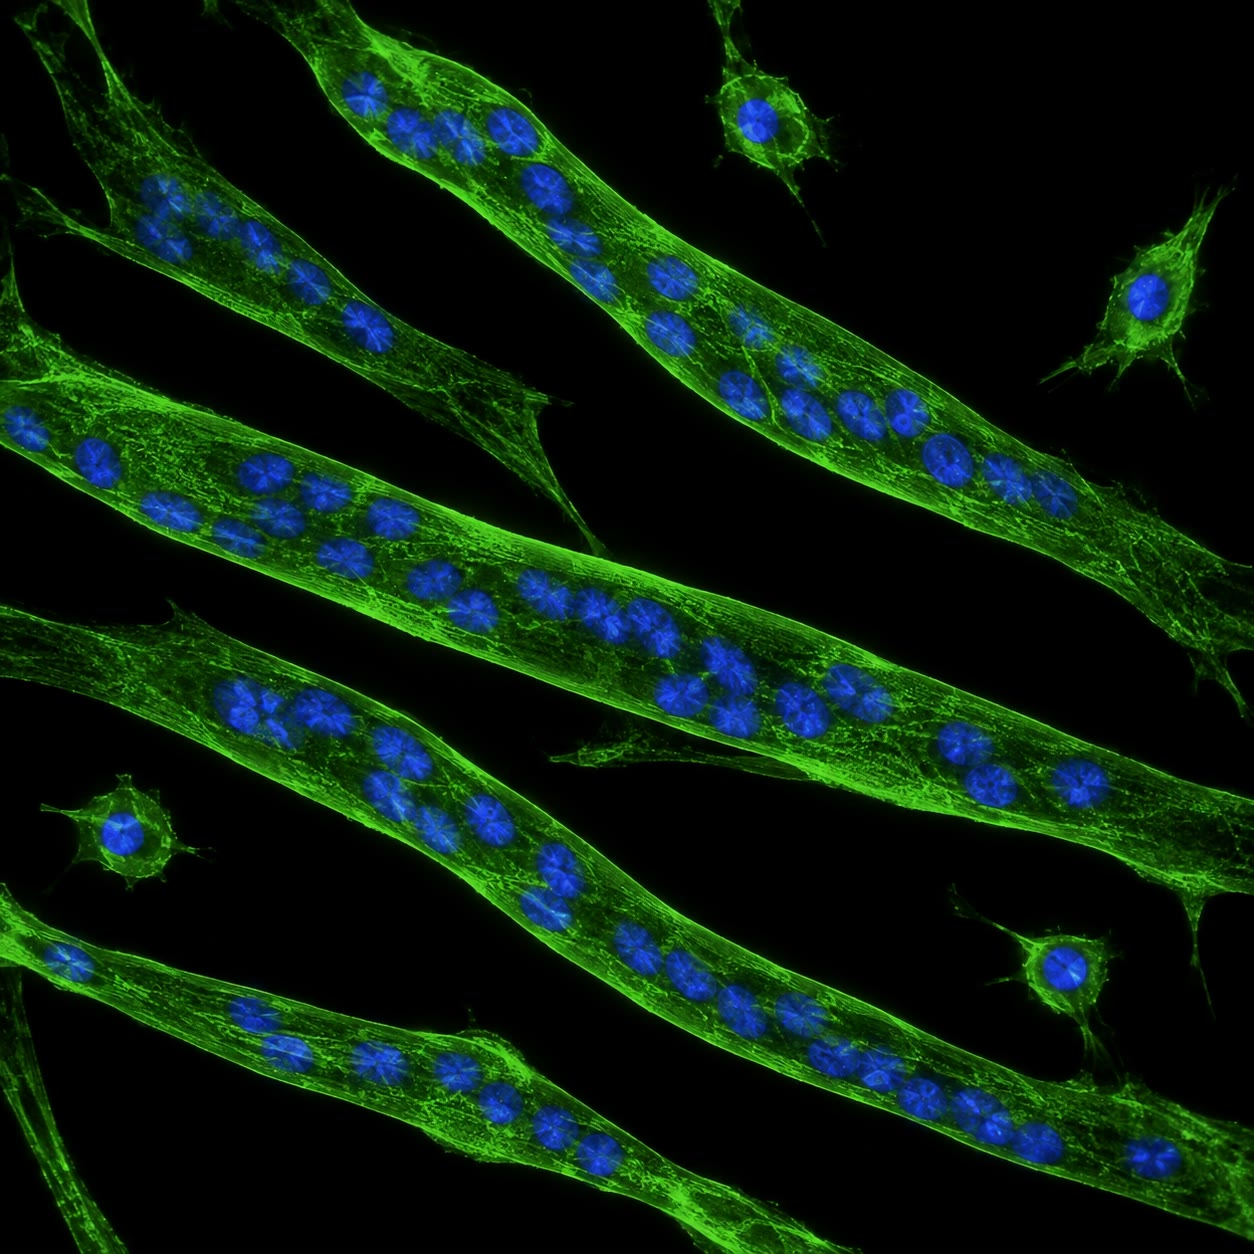
\includegraphics[width=0.44\linewidth]{images/book4/ai/b4-12-myotubes.jpg}\hspace{0.04\linewidth}
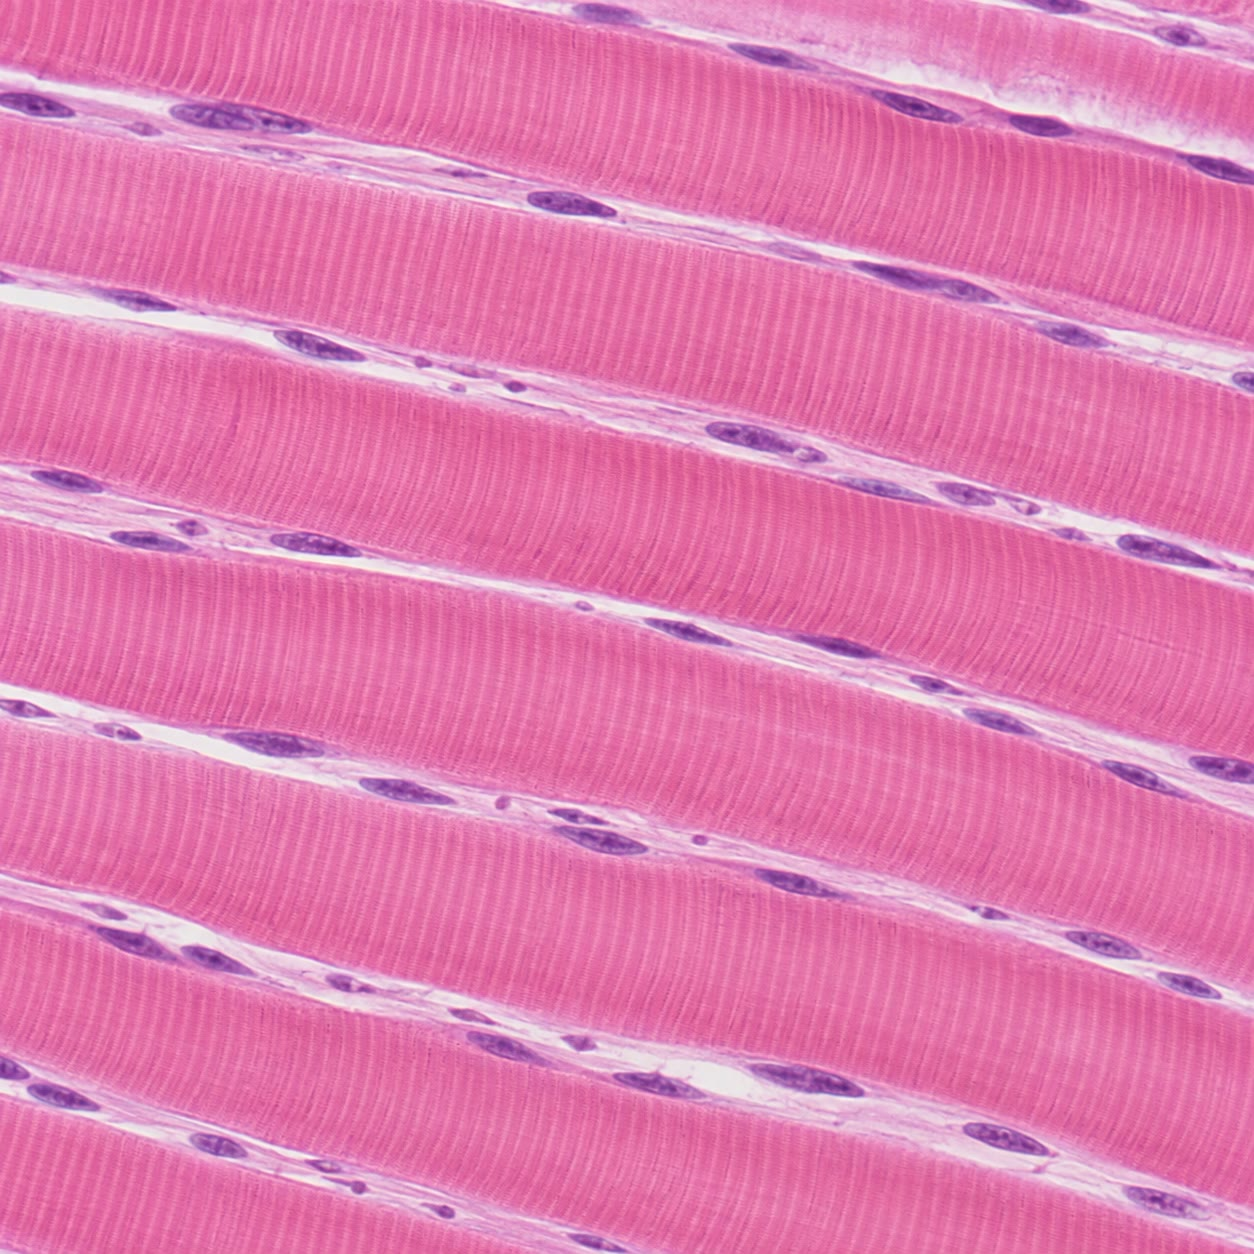
\includegraphics[width=0.44\linewidth]{images/book4/ai/b4-12-muscle-fibres.jpg}

{\small Links: \omterm{def:b2:cell-differentiation:myogenesis}{myotubes} in kweek, elk een versmolten cel met een rij kernen,
naast afzonderlijke \omterm{def:b2:cell-differentiation:myogenesis}{myoblasten} die nog niet zijn versmolten. Rechts: rijpe
vezels in lengteaanzicht, met als dwarsstrepen de zich herhalende
sarcomeren en met de kernen naar de rand gedrukt.}
\end{omfigure}

\begin{proposition}[MyoD: een hoofdschakelaar]\label{prop:b2:cell-differentiation:myod}
\index{hoofdregulator!MyoD}
\omterm{def:b2:cell-differentiation:myogenesis}{MyoD} is een \omterm{prop:b2:cell-differentiation:transcriptional}{transcriptiefactor} uit de helix-lus-helixfamilie. Het bindt,
als dimeer met een alomtegenwoordig partnereiwit, een sequentie van zes
basen (de E-box, CANNTG) in de regelgebieden van de spiergenen, rekruteert
enzymen die het chromatine openen, en schakelt de genen aan --- ook de
genen voor myogenine en voor \omterm{def:b2:cell-differentiation:myogenesis}{MyoD} zelf, en zo blijft de toestand bestaan.
Zijn activiteit wordt gepoort: in delende \omterm{def:b2:cell-differentiation:myogenesis}{myoblasten} houdt een remmend eiwit
(Id), geïnduceerd door groeifactoren, de partner vast en blijft \omterm{def:b2:cell-differentiation:myogenesis}{MyoD}
werkloos; wanneer de groeifactoren wegvallen, verdwijnt Id en treedt \omterm{def:b2:cell-differentiation:myogenesis}{MyoD}
in werking. Omdat \omterm{def:b2:cell-differentiation:myogenesis}{MyoD} volstaat om het spierprogramma op te leggen aan een
fibroblast, een vetcel of een zenuwcel, is het spierlot in zekere zin maar
één gen diep: de moeilijkheid om spier te worden ligt niet in weten hoe,
maar in het bevel krijgen.
\end{proposition}
\begin{proof}[Bewijsmateriaal]
Davis, Weintraub en Lassar (1987) brachten één enkel cDNA, geïsoleerd uit
\omterm{def:b2:cell-differentiation:myogenesis}{myoblasten}, over in gekweekte fibroblasten: de fibroblasten hielden op met
delen, versmolten tot \omterm{def:b2:cell-differentiation:myogenesis}{myotubes} en maakten spiereiwitten. Het gen kreeg de
naam \omterm{def:b2:cell-differentiation:myogenesis}{MyoD}. Zijn verwanten Myf5, myogenine en MRF4 werden op grond van
homologie gevonden; een muis die zowel \omterm{def:b2:cell-differentiation:myogenesis}{MyoD} als Myf5 mist, heeft geen
\omterm{def:b2:cell-differentiation:myogenesis}{myoblasten} en helemaal geen skeletspier, terwijl een muis zonder myogenine
\omterm{def:b2:cell-differentiation:myogenesis}{myoblasten} heeft die nooit versmelten.
\end{proof}

\begin{theorem}[Een zichzelf in stand houdende schakelaar]\label{thm:b2:cell-differentiation:switch}
\index{bistabiliteit}\index{positieve terugkoppeling!van een gen}
Zij $m$ de hoeveelheid van een factor die zijn eigen gen activeert met een
coöperatieve (sigmoïde) respons en wordt afgebroken met snelheid $k$:
\[
\frac{\mathrm{d}m}{\mathrm{d}t} = \frac{a\,m^{2}}{K^{2} + m^{2}} + b - k\,m,
\]
waarin $b$ een kleine basale synthese is. Voor geschikte $a$, $b$, $K$ en
$k$ heeft deze vergelijking \emph{twee} stabiele stationaire toestanden, een
lage bij ongeveer $b/k$ en een hoge bij ongeveer $a/k$, gescheiden door een
instabiele drempel: de cel is \emph{bistabiel}. Een voorbijgaand inductief
signaal dat $m$ boven de drempel duwt, stuurt de cel naar de hoge toestand,
waar ze blijft nadat het signaal is verdwenen; onder de drempel keert ze
terug naar de lage toestand. Dit is een geheugen gebouwd uit een
terugkoppelingslus, en daarom blijft een cel die eenmaal is vastgelegd dat
over de delingen heen en in afwezigheid van de inductor.
\end{theorem}
\begin{proof}
Stationaire toestanden voldoen aan $k m = a m^{2}/(K^{2} + m^{2}) + b$. Het
rechterlid is een sigmoïde die stijgt van $b$ tot $a + b$; het linkerlid is
een rechte door de oorsprong met helling $k$. Voor $b/k < K$ en $k$ klein
genoeg om de rechte het steile deel van de sigmoïde te laten snijden,
snijden de twee krommen elkaar drie keer: bij $m_{\text{laag}} \approx b/k$,
bij een tussenliggende $m_{\text{i}}$, en bij $m_{\text{hoog}} \approx (a +
b)/k$. Stabiliteit: onder $m_{\text{laag}}$ overtreft synthese de afbraak en
stijgt $m$; tussen $m_{\text{laag}}$ en $m_{\text{i}}$ overtreft afbraak de
synthese en valt $m$ terug; tussen $m_{\text{i}}$ en
$m_{\text{hoog}}$ overtreft synthese de afbraak en klimt $m$ naar
$m_{\text{hoog}}$; daarboven valt $m$ terug naar $m_{\text{hoog}}$.
De buitenste twee zijn dus stabiel, de middelste is instabiel en is de
drempel.
\end{proof}

\begin{omfigure}
\begin{tikzpicture}
\begin{axis}[
  width=0.74\linewidth, height=5.8cm,
  axis x line=bottom, axis y line=left,
  xmin=0, xmax=4, ymin=0, ymax=1.3,
  xlabel={niveau van de factor $m$ (relatief)}, ylabel={snelheid},
  xlabel style={font=\small, at={(axis description cs:0.5,-0.12)}, anchor=north},
  ylabel style={font=\small},
  tick label style={font=\small}, xtick={0,1,2,3,4}, ytick={0,0.5,1},
  legend style={font=\scriptsize, at={(0.03,0.97)}, anchor=north west, draw=none},
  clip=false,
]
\addplot[very thick, omDef, domain=0:4, samples=100] {x^2/(1+x^2) + 0.02};
\addlegendentry{synthese: $a m^2/(K^2 + m^2) + b$}
\addplot[very thick, omThm, domain=0:3.2, samples=2] {0.4*x};
\addlegendentry{afbraak: $k m$}
\fill[omDef] (axis cs:0.055,0.022) circle (2pt); \draw[gray] (axis cs:0.08,0.04) -- (axis cs:0.33,0.42); \node[font=\scriptsize, anchor=west] at (axis cs:0.35,0.45) {uit};
\draw[gray, thick] (axis cs:0.41,0.164) circle (2pt); \node[font=\scriptsize, anchor=west] at (axis cs:0.55,0.10) {drempel};
\fill[omDef] (axis cs:2.1,0.84) circle (2pt); \node[font=\scriptsize, anchor=north] at (axis cs:2.1,0.78) {aan};
\end{axis}
\end{tikzpicture}

{\small Een bistabiele schakelaar ($a = 1$, $K = 1$, $b = 0.02$, $k = 0.4$).
Synthese (sigmoïde) en afbraak (rechte) snijden elkaar drie keer: twee
stabiele toestanden, uit en aan, en daartussen een instabiele drempel.
Een signaal dat $m$ voorbij de drempel tilt, legt de cel blijvend vast in de
aan-toestand.}
\end{omfigure}

\section{De voltooide cel}

\begin{definition}[De spiervezel]\label{def:b2:cell-differentiation:fibre}
\index{sarcomeer}\index{myofibril}\index{sarcoplasmatisch reticulum}\index{T-tubulus}
Een skeletspiervezel is een cilinder van \qtyrange{10}{100}{\micro m}
doorsnede en tot tientallen centimeters lang, begrensd door het
\emph{sarcolemma}, met honderden kernen er vlak onder. Het inwendige is
gevuld met evenwijdige \emph{myofibrillen}, elk een keten van
\emph{sarcomeren} van \qty{2.5}{\micro m} lang: tussen twee Z-schijven
grijpen dunne filamenten van actine (met tropomyosine en troponine), aan de
Z-schijven verankerd, in dikke filamenten van myosine die in het midden
worden vastgehouden, en het overlappingspatroon geeft de dwarsstrepen. Rond
elke myofibril slaat een kantwerk van \emph{sarcoplasmatisch reticulum}
calcium op; \emph{transversale tubuli}, instulpingen van het sarcolemma,
lopen tussen de myofibrillen en voeren het elektrische signaal van het
oppervlak naar het inwendige. Mitochondriën vullen de tussenruimten, en het
cytoplasma bevat glycogeen, creatinefosfaat en, in rode vezels,
myoglobine. De cel is gebouwd voor één ding --- op bevel verkorten --- en de
machinerie van dat bevel is het onderwerp van
\cref{ch:b2:muscle-movement}.
\end{definition}

\begin{omfigure}
\begin{tikzpicture}[every node/.style={font=\scriptsize}]
  % a stretch of myofibril with two sarcomeres
  \foreach \s in {0,4.4} {
    \begin{scope}[xshift=\s cm]
      \draw[very thick, omThm] (0,-1.1) -- (0,1.1);
      \foreach \y in {-0.9,-0.5,-0.1,0.3,0.7} { \draw[thick, omDef] (0,\y) -- (1.6,\y); \draw[thick, omDef] (4.4,\y) -- (2.8,\y); }
      \foreach \y in {-0.7,-0.3,0.1,0.5,0.9} { \draw[line width=3pt, omExo!80!black] (1.0,\y) -- (3.4,\y); }
      \draw[gray] (2.2,-1.1) -- (2.2,1.1);
    \end{scope}
  }
  \draw[very thick, omThm] (8.8,-1.1) -- (8.8,1.1);
  \node[omThm, below] at (0,-1.15) {Z-schijf};
  \node[omThm, below] at (4.4,-1.15) {Z-schijf};
  \node[omThm, below] at (8.8,-1.15) {Z-schijf};
  \node[omDef, above] at (0.8,1.15) {dunne filamenten (actine)};
  \node[omExo!80!black, above] at (6.6,1.15) {dikke filamenten (myosine)};
  \node[gray, below] at (2.2,-1.15) {M-lijn};
  \draw[<->] (0,1.9) -- (4.4,1.9); \node[above] at (2.2,1.9) {één sarcomeer, \qty{2.5}{\micro m}};
  \draw[<->] (5.4,-1.6) -- (7.8,-1.6); \node[below] at (6.6,-1.6) {A-band (donker)};
  \draw[<->] (7.8,-1.6) -- (9.8,-1.6); \node[below] at (8.8,-1.6) {I-band (licht)};
\end{tikzpicture}

{\small Twee sarcomeren van een \omterm{def:b2:cell-differentiation:fibre}{myofibril}: dunne actinefilamenten, aan de
Z-schijven verankerd, grijpen in dikke myosinefilamenten die rond de M-lijn
zijn gecentreerd. De overlapping geeft de donkere A-band en de lichte I-band
van de dwarsstrepen.}
\end{omfigure}

\begin{proposition}[Vezeltypen]\label{prop:b2:cell-differentiation:types}
\index{spiervezeltypen}
Een spier is een mengsel van vezeltypen, deels bepaald door de lijn van de
\omterm{def:b2:cell-differentiation:myogenesis}{myoblast} en deels door de zenuw die de vezel innerveert. \emph{Langzame
oxidatieve} vezels (type I) hebben een traag myosine, veel mitochondriën en
haarvaten, en myoglobine --- rood, onvermoeibaar, gebouwd voor houding en
uithoudingsvermogen. \emph{Snelle glycolytische} vezels (type IIx) hebben
een snel myosine, weinig mitochondriën, veel glycogeen --- wit, krachtig,
binnen een minuut uitgeput. \emph{Snelle oxidatieve} vezels (type IIa)
liggen ertussen. De kuit van een sprinter bestaat vooral uit snelle vezels,
die van een marathonloper vooral uit langzame, en de verhoudingen zijn
erfelijk; maar het type ligt niet vast: een snelle spier kruisinnerveren
met een langzame zenuw, of maandenlange duurtraining, zet vezels om naar het
langzame type, omdat het patroon van zenuwimpulsen de genen voor de
myosine-isovormen en voor de mitochondriale biogenese schakelt. Een
gedifferentieerde cel behoudt haar identiteit als \omterm{def:b2:cell-differentiation:myogenesis}{spiervezel} en herziet
toch haar programma naargelang het gebruik.
\end{proposition}

\begin{example}[Groei en herstel]\label{ex:b2:cell-differentiation:satellite}
Een spier groeit bij de volwassene niet door vezels toe te voegen maar door
ze te vergroten: training voegt myofibrillen aan elke vezel toe, en
\emph{satellietcellen} versmelten ermee om de extra kernen te leveren die
een groter cytoplasma nodig heeft. Na een verwonding delen dezelfde cellen
zich, brengen ze \omterm{def:b2:cell-differentiation:myogenesis}{MyoD} opnieuw tot expressie, versmelten ze en herbouwen ze
het beschadigde segment binnen enkele weken --- het embryonale programma,
bij de volwassene opnieuw afgespeeld. Bij spierdystrofie missen de vezels
dystrofine, een eiwit dat de myofibrillen aan het membraan vastmaakt, en
scheuren ze tijdens de samentrekking; de satellietcellen herstellen ze
steeds opnieuw, tot de voorraad na jaren is uitgeput en bindweefsel de
plaats van de spier inneemt.
\end{example}

\begin{omfigure}
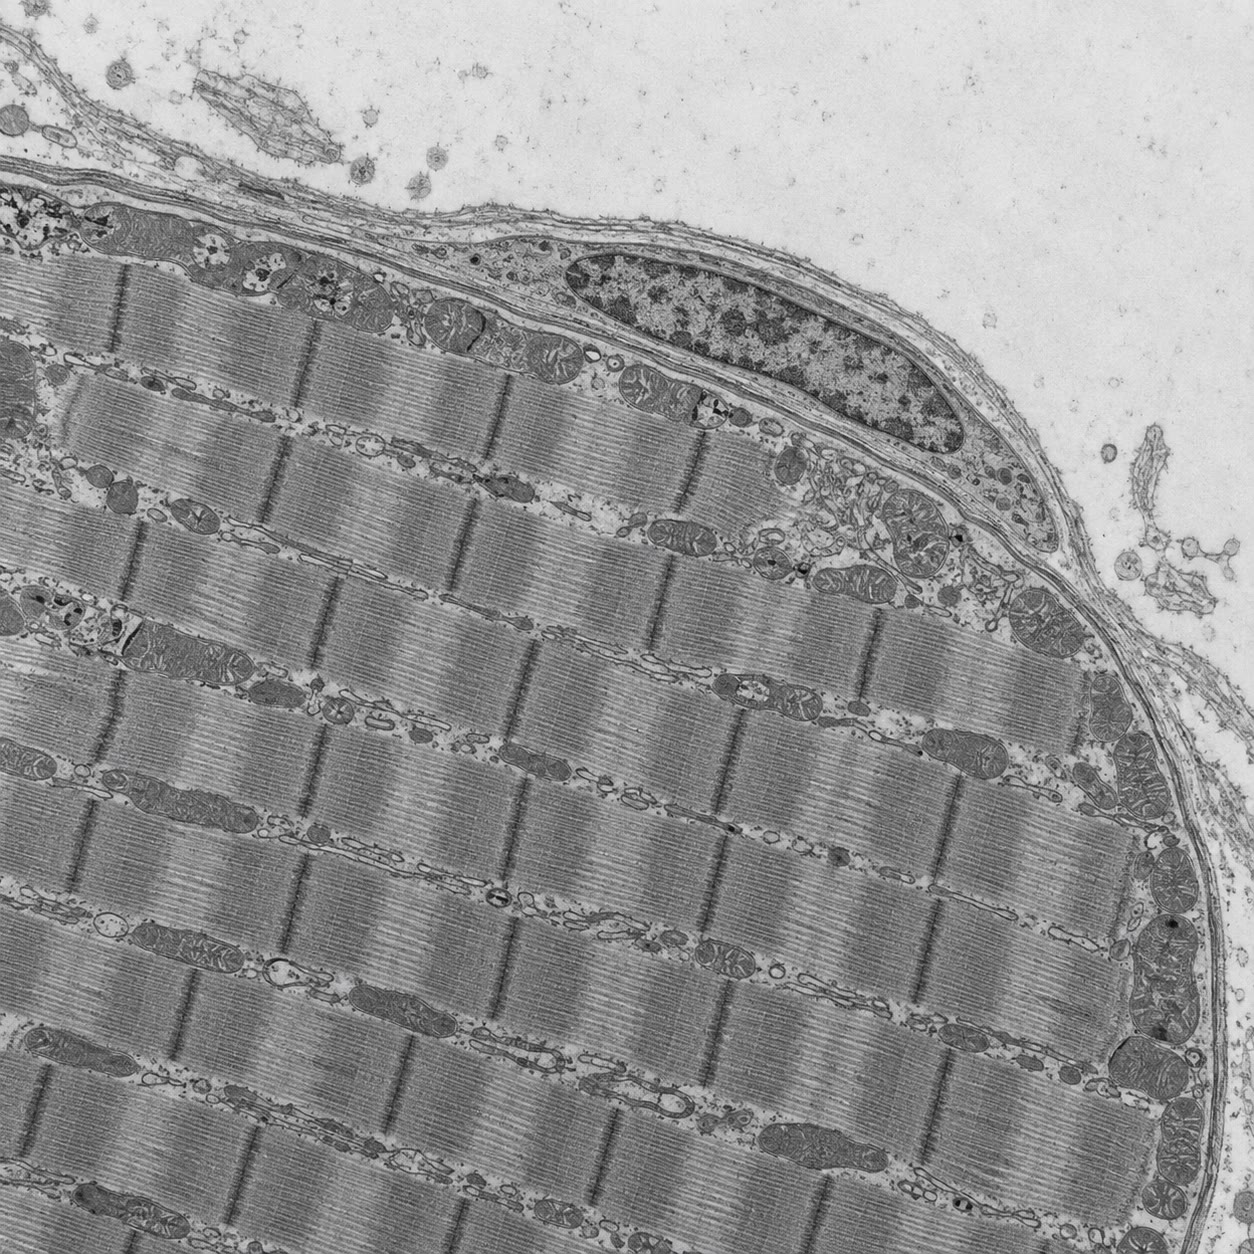
\includegraphics[width=0.42\linewidth]{images/book4/ai/b4-12-satellite-cell-tem.jpg}

{\small Een satellietcel onder de elektronenmicroscoop: een kleine
eenkernige cel, weggestopt tussen het membraan van een \omterm{def:b2:cell-differentiation:myogenesis}{spiervezel} en zijn
basale lamina --- de reserve aan \omterm{def:b2:cell-differentiation:myogenesis}{myoblasten} van de vezel.}
\end{omfigure}

\section{Opgaven}

\begin{exercise}[$\star$]\label{exo:b2:cell-differentiation:1}
Definieer \omterm{def:b2:cell-differentiation:differentiation}{differentiatie}, \omterm{def:b2:cell-differentiation:differentiation}{determinatie} en \omterm{def:b2:cell-differentiation:differentiation}{potentie}, en plaats de zygote,
een cel van de \omterm{def:b2:mammal-reproduction:implantation}{binnenste celmassa}, een satellietcel en een \omterm{def:b2:cell-differentiation:myogenesis}{spiervezel} op
de schaal van de \omterm{def:b2:cell-differentiation:differentiation}{potentie}.
\end{exercise}

\begin{exercise}[$\star$]\label{exo:b2:cell-differentiation:2}
Noem de stappen van de myogenese van somietcel tot \omterm{def:b2:cell-differentiation:myogenesis}{spiervezel}, met de
\omterm{prop:b2:cell-differentiation:transcriptional}{transcriptiefactor} die bij elke stap tot expressie komt.
\end{exercise}

\begin{exercise}[$\star$]\label{exo:b2:cell-differentiation:3}
Wat toonde de kerntransplantatie van Gurdon aan, en wat niet?
\end{exercise}

\begin{exercise}[$\star$]\label{exo:b2:cell-differentiation:4}
Noem de delen van een \omterm{def:b2:cell-differentiation:fibre}{sarcomeer} en zeg welke bewegen en welke niet wanneer
de vezel verkort.
\end{exercise}

\begin{exercise}[$\star\star$]\label{exo:b2:cell-differentiation:5}
Een vezel van \qty{20}{cm} lang heeft sarcomeren van \qty{2.5}{\micro m} en
een kern om de \qty{25}{\micro m} langs haar lengte. Hoeveel sarcomeren
liggen er in serie, en hoeveel kernen zijn er? Hoeveel \omterm{def:b2:cell-differentiation:myogenesis}{myoblasten}
versmolten om haar te maken?
\end{exercise}

\begin{exercise}[$\star\star$]\label{exo:b2:cell-differentiation:6}
Leg met de remmer Id uit waarom \omterm{def:b2:cell-differentiation:myogenesis}{myoblasten} niet versmelten zolang er FGF
aanwezig is, en voorspel wat er gebeurt met \omterm{def:b2:cell-differentiation:myogenesis}{myoblasten} die zo zijn
gemodificeerd dat ze Id constitutief maken.
\end{exercise}

\begin{exercise}[$\star\star$]\label{exo:b2:cell-differentiation:7}
Controleer in het schakelaarmodel met $a = 1$, $K = 1$, $b = 0.02$ en
$k = 0.4$ door invullen dat $m = 2.1$ dicht bij een stationaire toestand
ligt, bepaal bij benadering de lage stationaire toestand, en zeg wat er
gebeurt met een cel waarvan $m$ kortstondig tot $1$ wordt verhoogd en
die daarna met rust wordt gelaten.
\end{exercise}

\begin{exercise}[$\star\star$]\label{exo:b2:cell-differentiation:8}
In hetzelfde model wordt $k$ verhoogd tot $0.6$ (de factor wordt sneller
afgebroken). Toon grafisch of numeriek aan dat de hoge toestand verdwijnt.
Wat voorspelt dit voor een cel waarin \omterm{def:b2:cell-differentiation:myogenesis}{MyoD} wordt gedestabiliseerd?
\end{exercise}

\begin{exercise}[$\star\star$]\label{exo:b2:cell-differentiation:9}
Voorspel het \omterm{def:b2:meiosis-heredity:vocabulary}{fenotype} van een muis die (a) zowel \omterm{def:b2:cell-differentiation:myogenesis}{MyoD} als Myf5 mist,
(b) alleen myogenine mist, (c) alleen \omterm{def:b2:cell-differentiation:myogenesis}{MyoD} mist. Waarom is (c) bijna normaal?
\end{exercise}

\begin{exercise}[$\star\star\star$]\label{exo:b2:cell-differentiation:10}
Een fibroblast die met \omterm{def:b2:cell-differentiation:myogenesis}{MyoD} is getransfecteerd, wordt een \omterm{def:b2:cell-differentiation:myogenesis}{myotube}; een
levercel die met \omterm{def:b2:cell-differentiation:myogenesis}{MyoD} is getransfecteerd, niet. Stel een verklaring voor die
chromatine en \omterm{def:b2:vertebrate-development:induction}{competentie} betrekt, en een experiment om die te toetsen.
\end{exercise}

\begin{exercise}[$\star\star\star$]\label{exo:b2:cell-differentiation:11}
Duurtraining zet snelle vezels om naar langzame zonder hun genoom te
veranderen. Leg in termen van genexpressie uit hoe het vuurpatroon van de
zenuw dit kan doen, en waarom de vezels toch skeletspier blijven en nooit,
zeg, kraakbeen worden.
\end{exercise}

\begin{exercise}[$\star\star\star$]\label{exo:b2:cell-differentiation:12}
``Een gedifferentieerde cel onthoudt wat ze is met een schakeling, niet met
een \omterm{def:b2:genome-diversification:mutation}{mutatie}.'' Bespreek dit aan de hand van de bistabiele schakelaar, het
chromatine, en het feit dat het terugzetten door Gurdon en door Yamanaka
mogelijk maar inefficiënt is.
\end{exercise}

\section{Vraagstuk: een spier gebouwd en herbouwd}

\begin{problem}[{Weekendvraagstuk --- een spier gevolgd van somiet tot vezel
en door een verwonding heen: de aantallen myoblasten, versmeltingen en
kernen, de bistabiele schakelaar geanalyseerd, een herstel getimed en
training gekwantificeerd, met als besluit het aantal kernen van de vezel,
de drempel van de schakelaar en de hersteltijd}]
\label{pb:b2:cell-differentiation:1}
Een dijspier van een volwassene telt \num{500000} vezels, elk
\qty{20}{cm} lang en \qty{60}{\micro m} in doorsnede, met één kern per
\qty{25}{\micro m} lengte; sarcomeren zijn \qty{2.5}{\micro m} lang.
Embryonale \omterm{def:b2:cell-differentiation:myogenesis}{myoblasten} delen zich om de \qty{12}{h} zolang er FGF aanwezig
is. Schakelaarmodel: $a = 1$, $K = 1$, $b = 0.02$, $k
= 0.4$. Na een verwonding die \qty{10}{\%} van de lengte van elke vezel
vernietigt, delen de satellietcellen van het beschadigde segment (\num{4}
per millimeter vezel) zich een tijdlang om de \qty{18}{h} en versmelten ze
daarna.

\medskip
\noindent\textbf{Deel I --- De vezel.}
\begin{enumerate}
  \item Bereken het aantal sarcomeren in serie in één vezel en het aantal
        kernen.
  \item Hoeveel \omterm{def:b2:cell-differentiation:myogenesis}{myoblasten} versmolten om één vezel te maken? En de hele
        spier?
  \item Bereken het volume van één vezel en van de spier (in liter).
  \item Schat het volume cytoplasma dat door één kern wordt bediend, en
        vergelijk met een gewone cel van \qty{2000}{\micro m^3}.
  \item Waarom liggen de kernen aan de rand van een rijpe vezel?
  \item De \omterm{def:b2:cell-differentiation:myogenesis}{myoblasten} van de spier stammen af van \num{2000} somietcellen.
        Hoeveel verdubbelingen, en hoeveel dagen, hadden ze nodig om het
        aantal van vraag 2 te bereiken?
\end{enumerate}

\medskip
\noindent\textbf{Deel II --- De schakelaar.}
\begin{enumerate}[resume]
  \item Schrijf de voorwaarde voor een stationaire toestand op en toon aan
        dat $m \approx
        0.055$ eraan voldoet.
  \item Toon aan dat $m \approx 2.1$ eraan voldoet.
  \item Toon aan dat er een derde oplossing is bij ongeveer $m = 0.41$, en
        leg aan de hand van het teken van $\mathrm{d}m/\mathrm{d}t$ aan
        weerszijden uit dat die instabiel is.
  \item Een puls van inductor verhoogt $m$ tot $0.6$; een andere tot $0.3$.
        Wat is het lot van elke cel?
  \item De basale synthese $b$ wordt door een \omterm{def:b2:genome-diversification:mutation}{mutatie} verhoogd tot $0.4$.
        Toon aan dat de lage toestand verdwijnt. Wat doet de cel?
  \item Leg uit hoe dit model verklaart dat de vastlegging een celdeling
        overleeft, en wat er bij elke deling voor $m$ moet gelden.
\end{enumerate}

\medskip
\noindent\textbf{Deel III --- Herstel.}
\begin{enumerate}[resume]
  \item Hoeveel satellietcellen draagt één vezel, en hoeveel kernen moeten
        na de verwonding worden vervangen?
  \item Hoeveel verdubbelingen moeten de satellietcellen doormaken om die
        te leveren, en hoelang duurt dat?
  \item Vergelijk met de waargenomen twee tot drie weken voor het herstel,
        en zeg wat die tijd nog meer omvat.
  \item Waarom moeten de satellietcellen \omterm{def:b2:cell-differentiation:myogenesis}{MyoD} opnieuw tot expressie brengen
        voordat ze versmelten, en waarom moeten ze eerst ophouden met delen?
  \item Elke herstelronde verbruikt een deel van de satellietcellen. Als de
        voorraad per verwonding met \qty{5}{\%} daalt, na hoeveel
        verwondingen is hij dan gehalveerd?
  \item Hoeveel satellietcellen per vezel blijven er over na twintig zulke
        verwondingen?
  \item Leg uit waarom een dystrofische spier, waarvan de vezels bij elke
        samentrekking scheuren, na jaren door bindweefsel wordt vervangen.
\end{enumerate}

\medskip
\noindent\textbf{Deel IV --- Training.}
\begin{enumerate}[resume]
  \item Training verdikt elke vezel tot \qty{80}{\micro m}. Met welke factor
        groeit het volume van de vezel, en hoeveel extra kernen moeten de
        satellietcellen leveren als de verhouding van vraag 4 behouden
        blijft?
  \item Bereken het nieuwe volume van de spier.
  \item Duurtraining zet \qty{30}{\%} van de snelle vezels om in langzame.
        Wat is er in die vezels veranderd en wat niet?
  \item Leg uit waarom een volwassen spier groter wordt door groei van vezels
        en niet door toevoeging van vezels, met het gegeven dat vezels zich
        niet delen.
  \item Een geneesmiddel blokkeert het versmelten van satellietcellen.
        Voorspel de reactie van de spier op training en op een verwonding.
  \item Formuleer het resultaat: het aantal kernen van de vezel, de drempel
        van de schakelaar, en de tijd die satellietcellen nodig hebben om de
        kernen voor een herstel te leveren.
\end{enumerate}
\end{problem}
